\Chapter{Numerical Experiment}
\section{When beta is not accurate?}
Examples to show for certain functions beta needs to be updated. 
\section{Option Pricing}
Option Pricing has always been a challenging topic in financial mathematics.
Add some reasons?\\
Hence it became a good application for our QMC algorithm.
Here we are going to demonstrate several examples of pricing different options with ccontrol variates.

\subsection{Asian Option}
There are two types of asian options, depends on which types of mean you want to use.For this example we take arithematic mean asian call option as our target function, whose payoff function is:
\[ C_{T}^{Amean} = \max\Big(\frac{1}{d}\sum_{j=1}^{d}S(jT/d)-K, 0\Big)\]
\begin{table}[H]
    \centering
	\begin{tabular}{lllllll}
		\toprule
		 S0 & K & TimeVector & r & volatility & abstol & reltol \\
		\midrule
		 120  & 130 & 1/52:1/52:16/52 & 0.01 & 0.5 & 1e-3 & 0\\ 
		\bottomrule
	\end{tabular}
	\caption{Parameter Setup for Up and In Barrier Call Option}
\end{table}
\begin{table}[H]
    \centering
	\begin{tabular}{  
		r>{\columncolor[gray]{.8}} r >{\color{white}\columncolor[gray]{.2}}r 
		r>{\columncolor[gray]{.8}} r >{\color{white}\columncolor[gray]{.2}}r} 
	\toprule
	\multicolumn{3}{c}{Sample Size}
		&\multicolumn{3}{c}{Time Cost} \\
	\cmidrule(r){1-6}
	 cubSobol&cv\_old&cv\_new
	 &cubSobol&cv\_old&cv\_new\\
        \midrule
		 65535&8192&9011
		&0.2783&0.1034&0.0673\\
	\bottomrule
	\end{tabular}
	\caption{Results of cubSobol, cv\_old and cv\_new with Asian Option}
\end{table}
Figure~\ref{} shows decrease rate the walsh coefficients for the target function and control variates in this example. 
\begin{figure}[H]
    \caption{}
    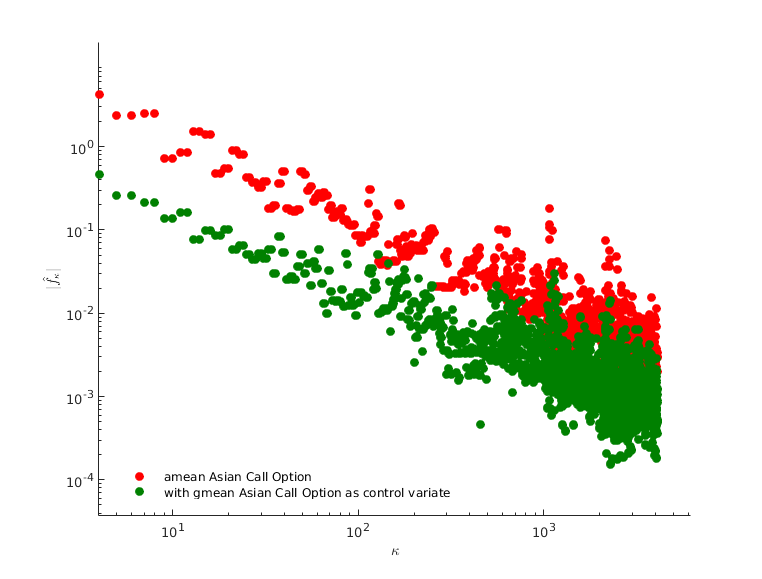
\includegraphics[width=0.8\textwidth]{figures/cvEx1.eps}
\end{figure}

\subsection{Barrier Option}
We will take up and in barrier call option as an example.
Here is the payoff function for up and in barrier call option.
\[ C_{T}^{U\&I} = (S_T-K)^+1_{ \{\max S_t \geq Barrier\}} \]
From the payoff function it is naturally to consider european call option as 
control variates. Since if we take the barrier same as strike price, then this is just an european call option.  
Table~\ref{BarrierPara} shows our setup for the barrier option.
\begin{table}[H]
    \centering
	\begin{tabular}{lllllll}
		\toprule
		 S0 & K & TimeVector & r & volatility & abstol & reltol \\
		\midrule
		 120  & 130 & 1/52:1/52:16/52 & 0.01 & 0.5 & 1e-3 & 0\\ 
		\bottomrule
	\end{tabular}
	\caption{Parameter Setup for Up and In Barrier Call Option}
    \label{tb:BarrierPara}
\end{table}
\begin{table}[H]
    \centering
	\begin{tabular}{l
		r>{\columncolor[gray]{.8}} r >{\color{white}\columncolor[gray]{.2}}r 
		r>{\columncolor[gray]{.8}} r >{\color{white}\columncolor[gray]{.2}}r} 
	\toprule
	Barrier &\multicolumn{3}{c}{Sample Size}
		&\multicolumn{3}{c}{Time Cost} \\
	\cmidrule(r){2-7}
	 &cubSobol&cv\_old&cv\_new
	 &cubSobol&cv\_old&cv\_new\\
        \midrule
	140  & 524288&78643& 65535
	     & 1.874& 0.5016&0.2743 \\ 
	135  & 524288& 5802&6963
	     & 1.959& 0.0781&0.0519 \\ 
	130  & 524288& 1024&1024
	     & 1.876& 0.0270 & 0.0199 \\
	\bottomrule
	\end{tabular}
	\caption{Results of cubSobol, cv\_old and cv\_new with Barrier Option}
\end{table}
We then took three different barrier as listed in table~\ref{tb:BarrierResults},
then we compared both oringinal cubSobol algorithm and the one with our modification as described in Chapter 4. \\
We can see from the results in table~\ref{tb:BarrierResults}

